\documentclass[10pt]{article}
\usepackage{amsmath}
\usepackage{paralist}
\usepackage{setspace}
\usepackage{listings}
\usepackage{graphicx}
\usepackage[english]{babel}
\usepackage{geometry}
\usepackage{subcaption}
\usepackage[utf8]{inputenc}
\usepackage{listings}

\begin{document}
\lstset{
	language=Matlab,
	basicstyle=\footnotesize,
	frame=tb,
	xleftmargin=.2\textwidth,
	xrightmargin=.2\textwidth
}
\onehalfspacing
\begin{titlepage}
\begin{center}
% Oberer Teil der Titelseite:


\textsc{\LARGE University Oldenburg}\\[1.5cm]

\textsc{\Large Wind Physics Measurement Project}\\[0.5cm]


% Title
\newcommand{\HRule}{\rule{\linewidth}{0.5mm}}
\HRule \\[0.4cm]
{ \huge \bfseries Exercise 1 - Handling and preprocessing of measurement data}\\[0.4cm]

\HRule \\[1.5cm]

% Author and supervisor
\begin{minipage}{0.4\textwidth}
\begin{flushleft} \large
\emph{Author:}\\
Jan \textsc{K\"amper}\\
Florian \textsc{B\"orgel}
\end{flushleft}
\end{minipage}
\hfill
\begin{minipage}{0.4\textwidth}
\begin{flushright} \large
\emph{Supervisor:} \\
Matthias \textsc{Wächter}
\end{flushright}
\end{minipage}
\\[3cm]
\vfill



% Unterer Teil der Seite
{\large \today}

\end{center}

\end{titlepage}
\tableofcontents
\newpage
\section*{Introduction}
The goal of this exercise was to perform some basic processing steps of raw measurement data from a met mast. The data used here originates from the FINO 1 platform in the German Northsea which includes two wind vanes at heights of 33m and 90m as well as eight anemometers at heights $33m, 40m, 50m, 60m, 70m, 80m, 90m$ and $100m$. The given time period of 1-Hertz data is of one month (January 2013). The six tasks described in the following reach from standard data treatment to a first simple analysis by looking at the increment probability density function in terms of wind speed fluctuations.

\section{Importing Data into Matlab}
The first step was loading the data given as ASCII file into Matlab-readable data structures. For the first task we used the function \textit{readtable()} to import the data with the corresponding delimiter as parameter. The advantage of using a table structure instead of a matrix is that the column headers like 'u100' or 'Time' are stored within the data structure. In this way we can easily separate the actual measurment data from the time stamp by splitting the table up in two matrices. \\
\begin{lstlisting}
time_stamp = raw_data{:, {'Time'}};
raw_data = raw_data{:, {'d90', 'd33', 'u100', 'u90', 'u80', ...
'u70', 'u60', 'u50', 'u40', 'u33'}};
\end{lstlisting}

\section{Marking invalid data}
In order to mark invalid data which is provided with a value of $-999$ by the measurement system the next section of our Matlab script converts all values $-999$ to $NaN$. Matlab checks if there is any invalid Data and replaces it with $NaN$. This is necessary for some remaining tasks when means and standard deviations will be computed which must not consider invalid values.\\
\begin{lstlisting}
raw_data(raw_data==-999) = NaN;
\end{lstlisting}

\section{Generating continuous time axis}
To avoid gaps in the time axis we first converted our time $t$ with \textit{datenum()} to a numeric value. The numeric values represent elapsed time in units of days. Hence, 1 second corresponds to the fraction of  $\frac{1}{24\cdot60\cdot60}$ of these numeric values. So after multiplication with the inverse value of that and rounding we obtain unique integer IDs for every occuring timestamp. 
Afterwards, we created the continuous time axis, by initializing a vector with length equaling exactly the number of seconds in January. 
Then, we filled the corrected data matrix $data\_pp$ with $NaN$ values and overwrote the file with our existing data at all indices where values are given.\\
\begin{lstlisting}
disp('Creating continous time axis')
tnew=[t(1):1:t(end)]';
data_pp = NaN(length(tnew),10);
disp('Writing preprocessed Data...')
for i = 1:length(raw_data(:,1))
    data_pp(t(i)-t(1)+1, :) = raw_data(i, :);
end
time = (1:length(data_pp))';
data_pp = [time, data_pp];
save('data_pp.mat', 'data_pp', 'raw_data');
clear;
\end{lstlisting}

\section{Computing 10min means and stddev}
This task is a first step of statistical analysis of the given data. We split our time axis into intervals of 600 seconds and for each interval we compute the mean and standard deviation for all ten variables for the . Invalid data can be ignored by using the commands \textit{nanmean()} and \textit{nanstd()}. Considering the wind directions a special treatment of the angles is required in order to handle the circular data, e.g. the mean value of $350^{\circ}$ and $10^{\circ}$ is not $180^{\circ}$ but $0^{\circ}$. Some trigonometric functions can be employed in order to cope with this.\\

We plotted the ten minute means of the $u100$ anemometer for one specific day and added the standard deviation to it. The outcome is depicted in figure \ref{fig:means}.
\begin{figure}[htb!]
  \centering
  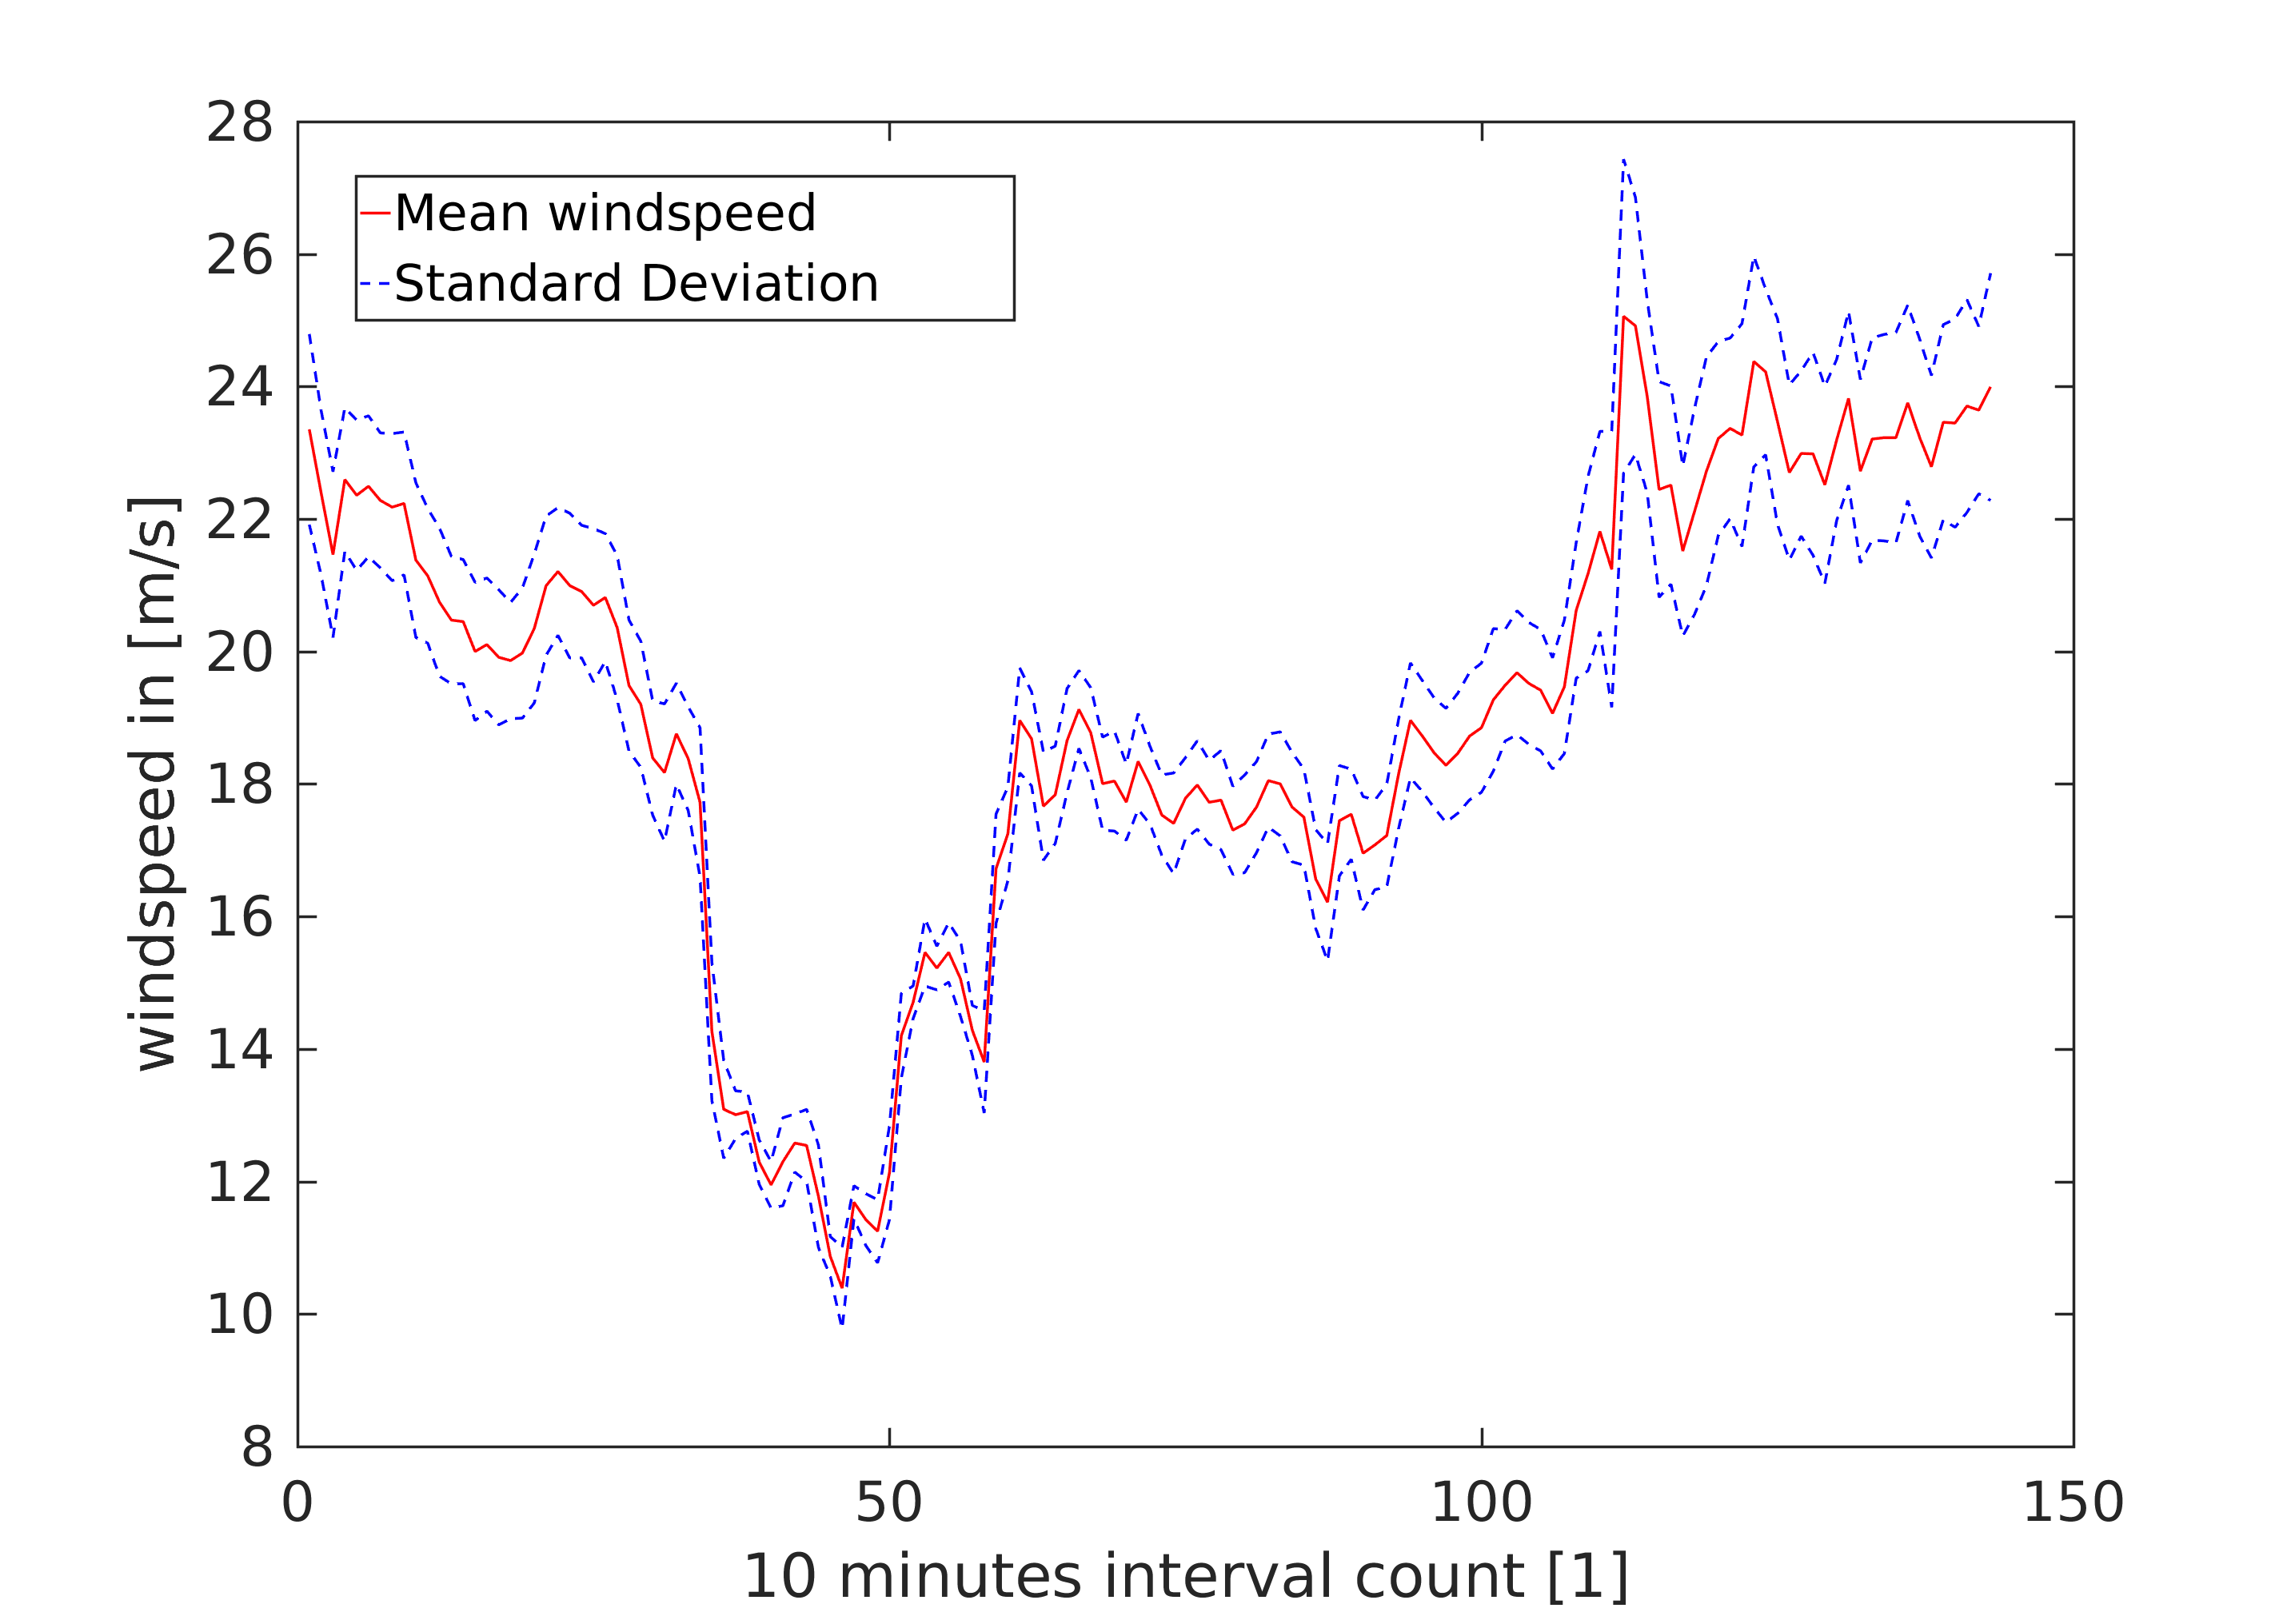
\includegraphics[width=1\linewidth]{../Plots/mean_interval_withstd.png}
  \caption{10 minute intervals for Jan 30th 2013}
  \label{fig:means}
\end{figure}

For this specific day we observe a very strong fluctuation of the wind over the day. During the early morning the wind is steadily strong with windspeeds greater then $20 m/s$ then drops by almost $60 \%$ untill 8am, then picks up again to reach a maximum of around $24 m/s$ in the evening. Indeed a very stormy day. The mean value and standard deviation are obivously not stationary because then mean is high in the morning and evening and low inbetween. The fluctuations and thus the standard deviation picks up in the evening and therefore is also not stationary.

\section{Extreme values}
In this task we looked for so called spikes. These are extremely high or low values within their immediate neighborhood, here 10 minutes intervals. A standard procedure to define spikes is to find values which exceed $[\mu - 5\sigma , \mu+5\sigma]$ in these intervals where $\mu$ is the mean and $\sigma$ is the standard deviation. 

Two such intervals and contained spikes where found by our algorithm and are plotted in figures \ref{fig:spikePhys} and \ref{fig:spikeUnphys}. The first shows a spike which appears to be of unphysical nature due to a relatively monotonous behaviour with only small fluctuations except one single value. This single value is below the $\mu-5\sigma$ line. So here we could talk of a measurement error. The second plot however exhibits a more physical behaviour. Here we have stronger fluctuation overall and the spike which is below $\mu-5\sigma$ matches the fluctuational pattern because the values before and after the spike also deviate a lot from the mean over a considerable period of time.

\begin{figure}[htb!]
  \centering
  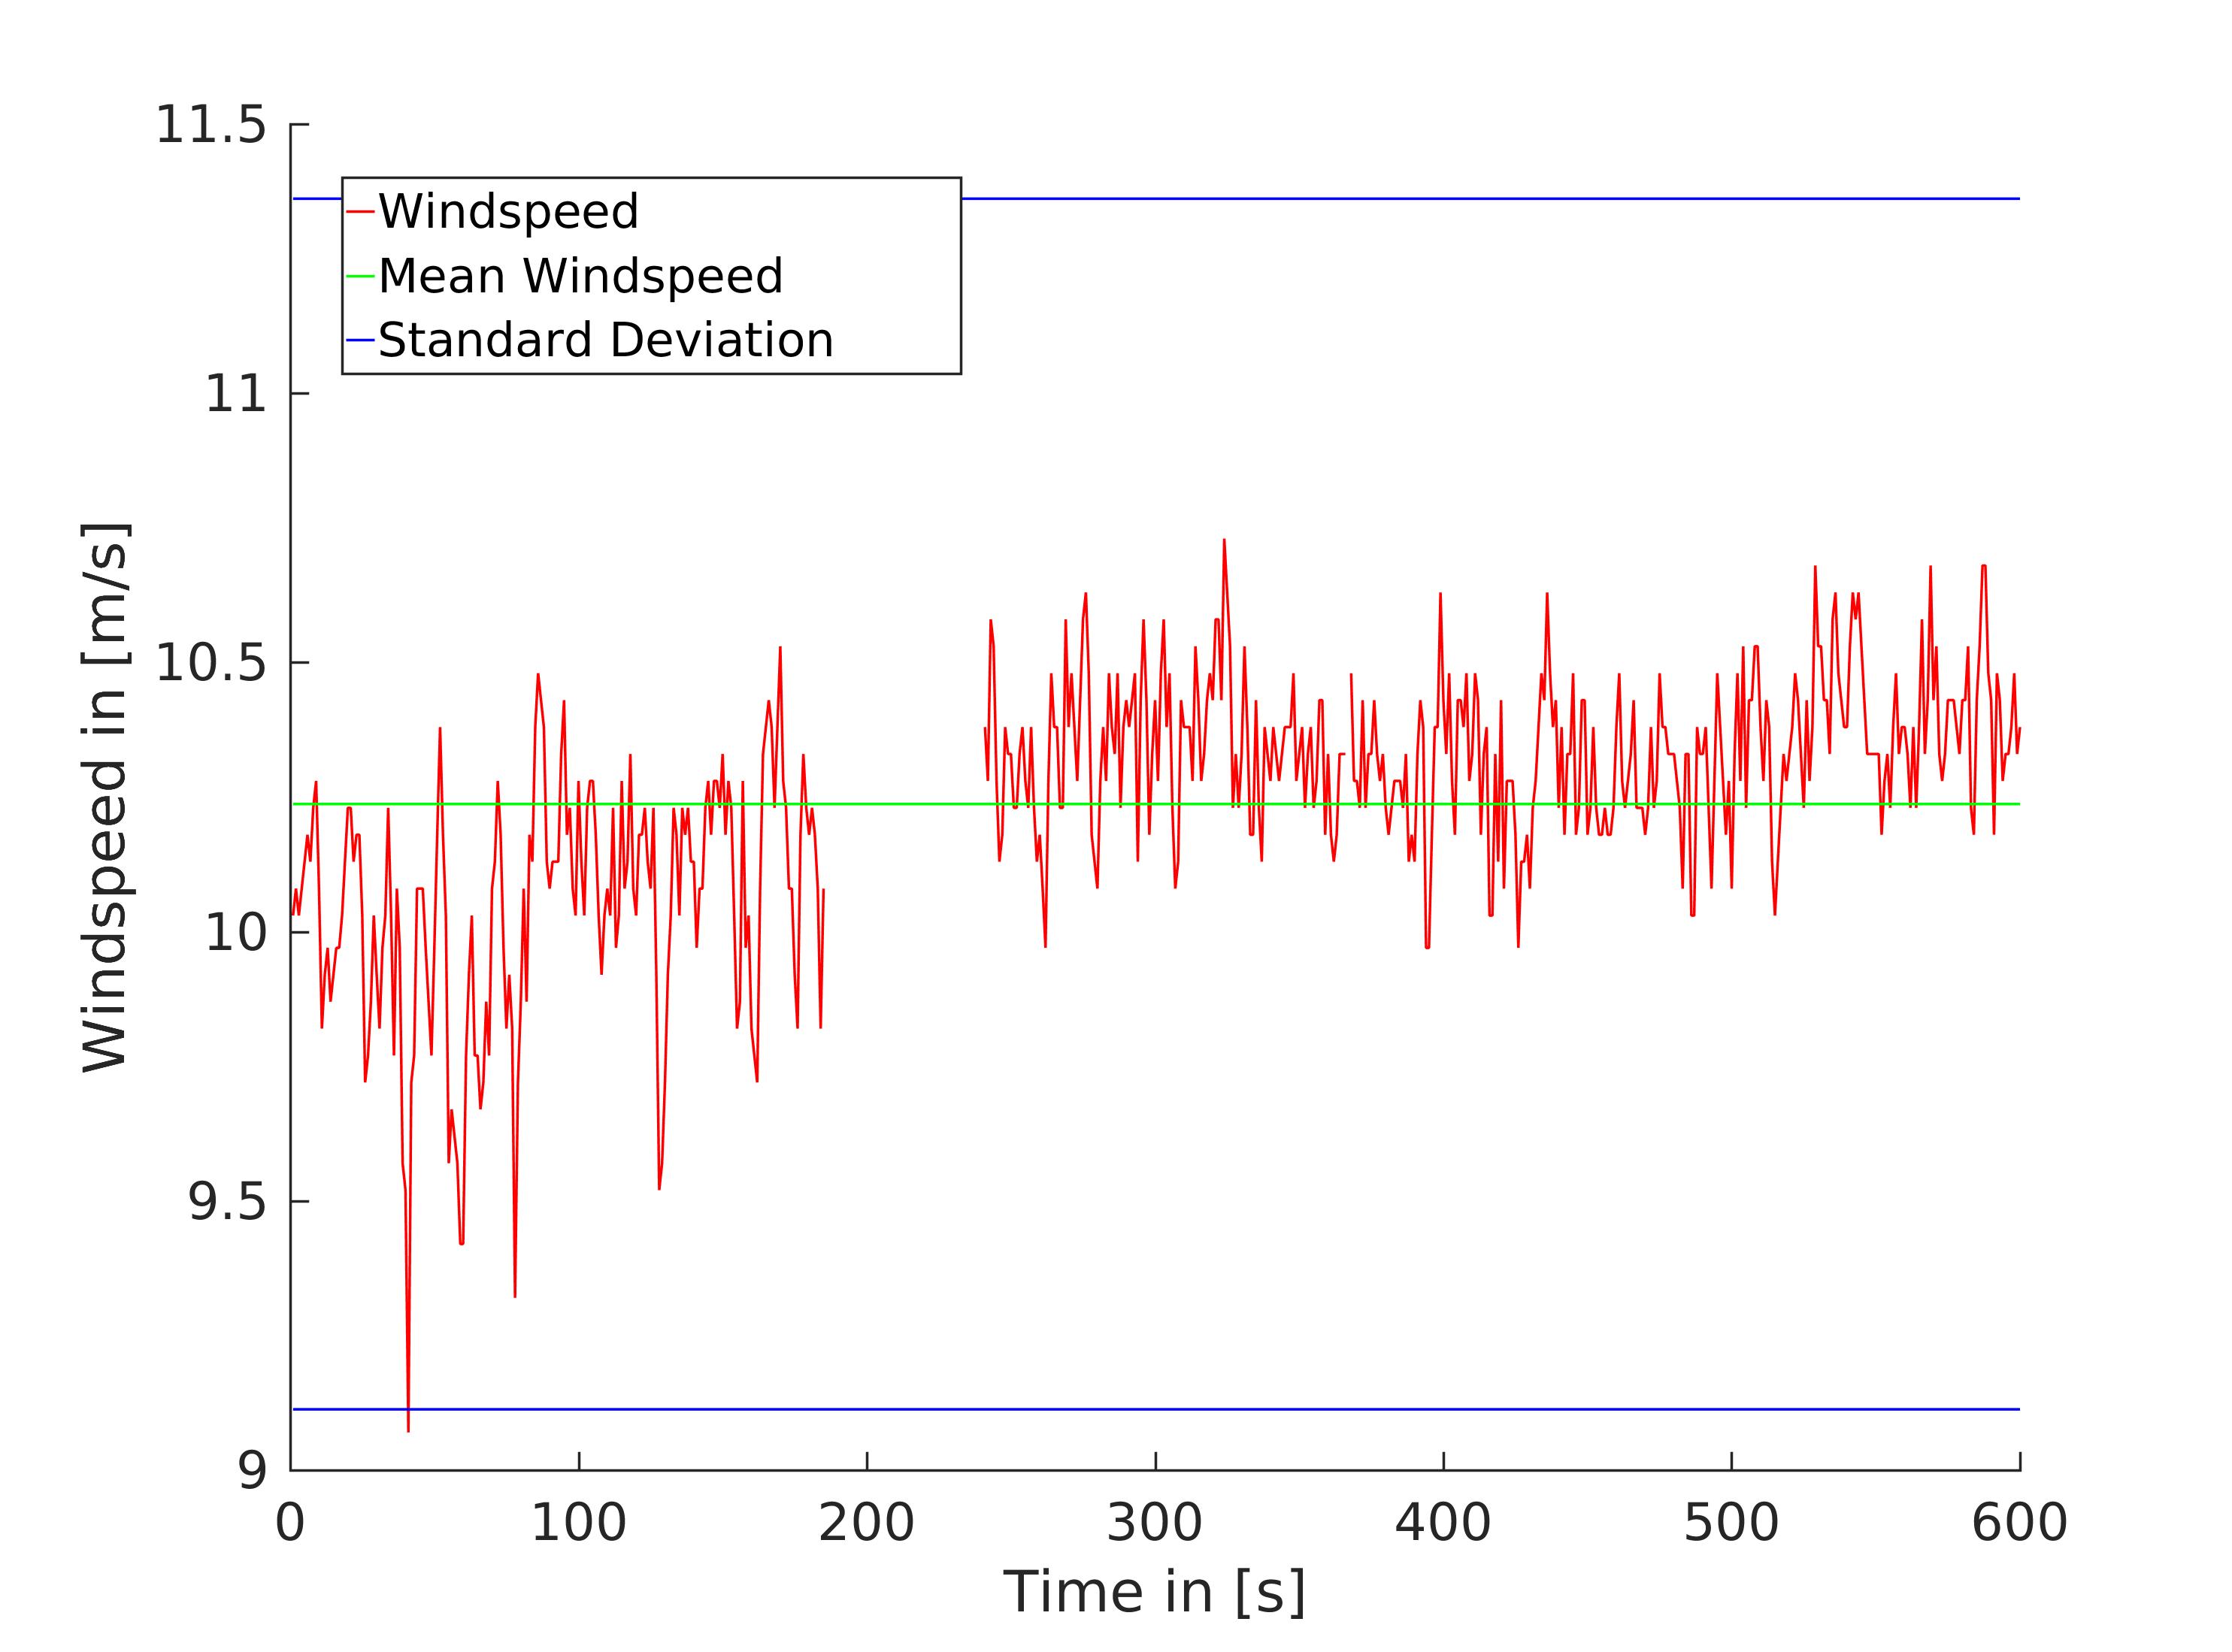
\includegraphics[width=1\linewidth]{../Plots/spikesintervall942.png}
  \caption{Physical cause}
    \label{fig:spikePhys}
\end{figure}
\begin{figure}[htb!]
  \centering
  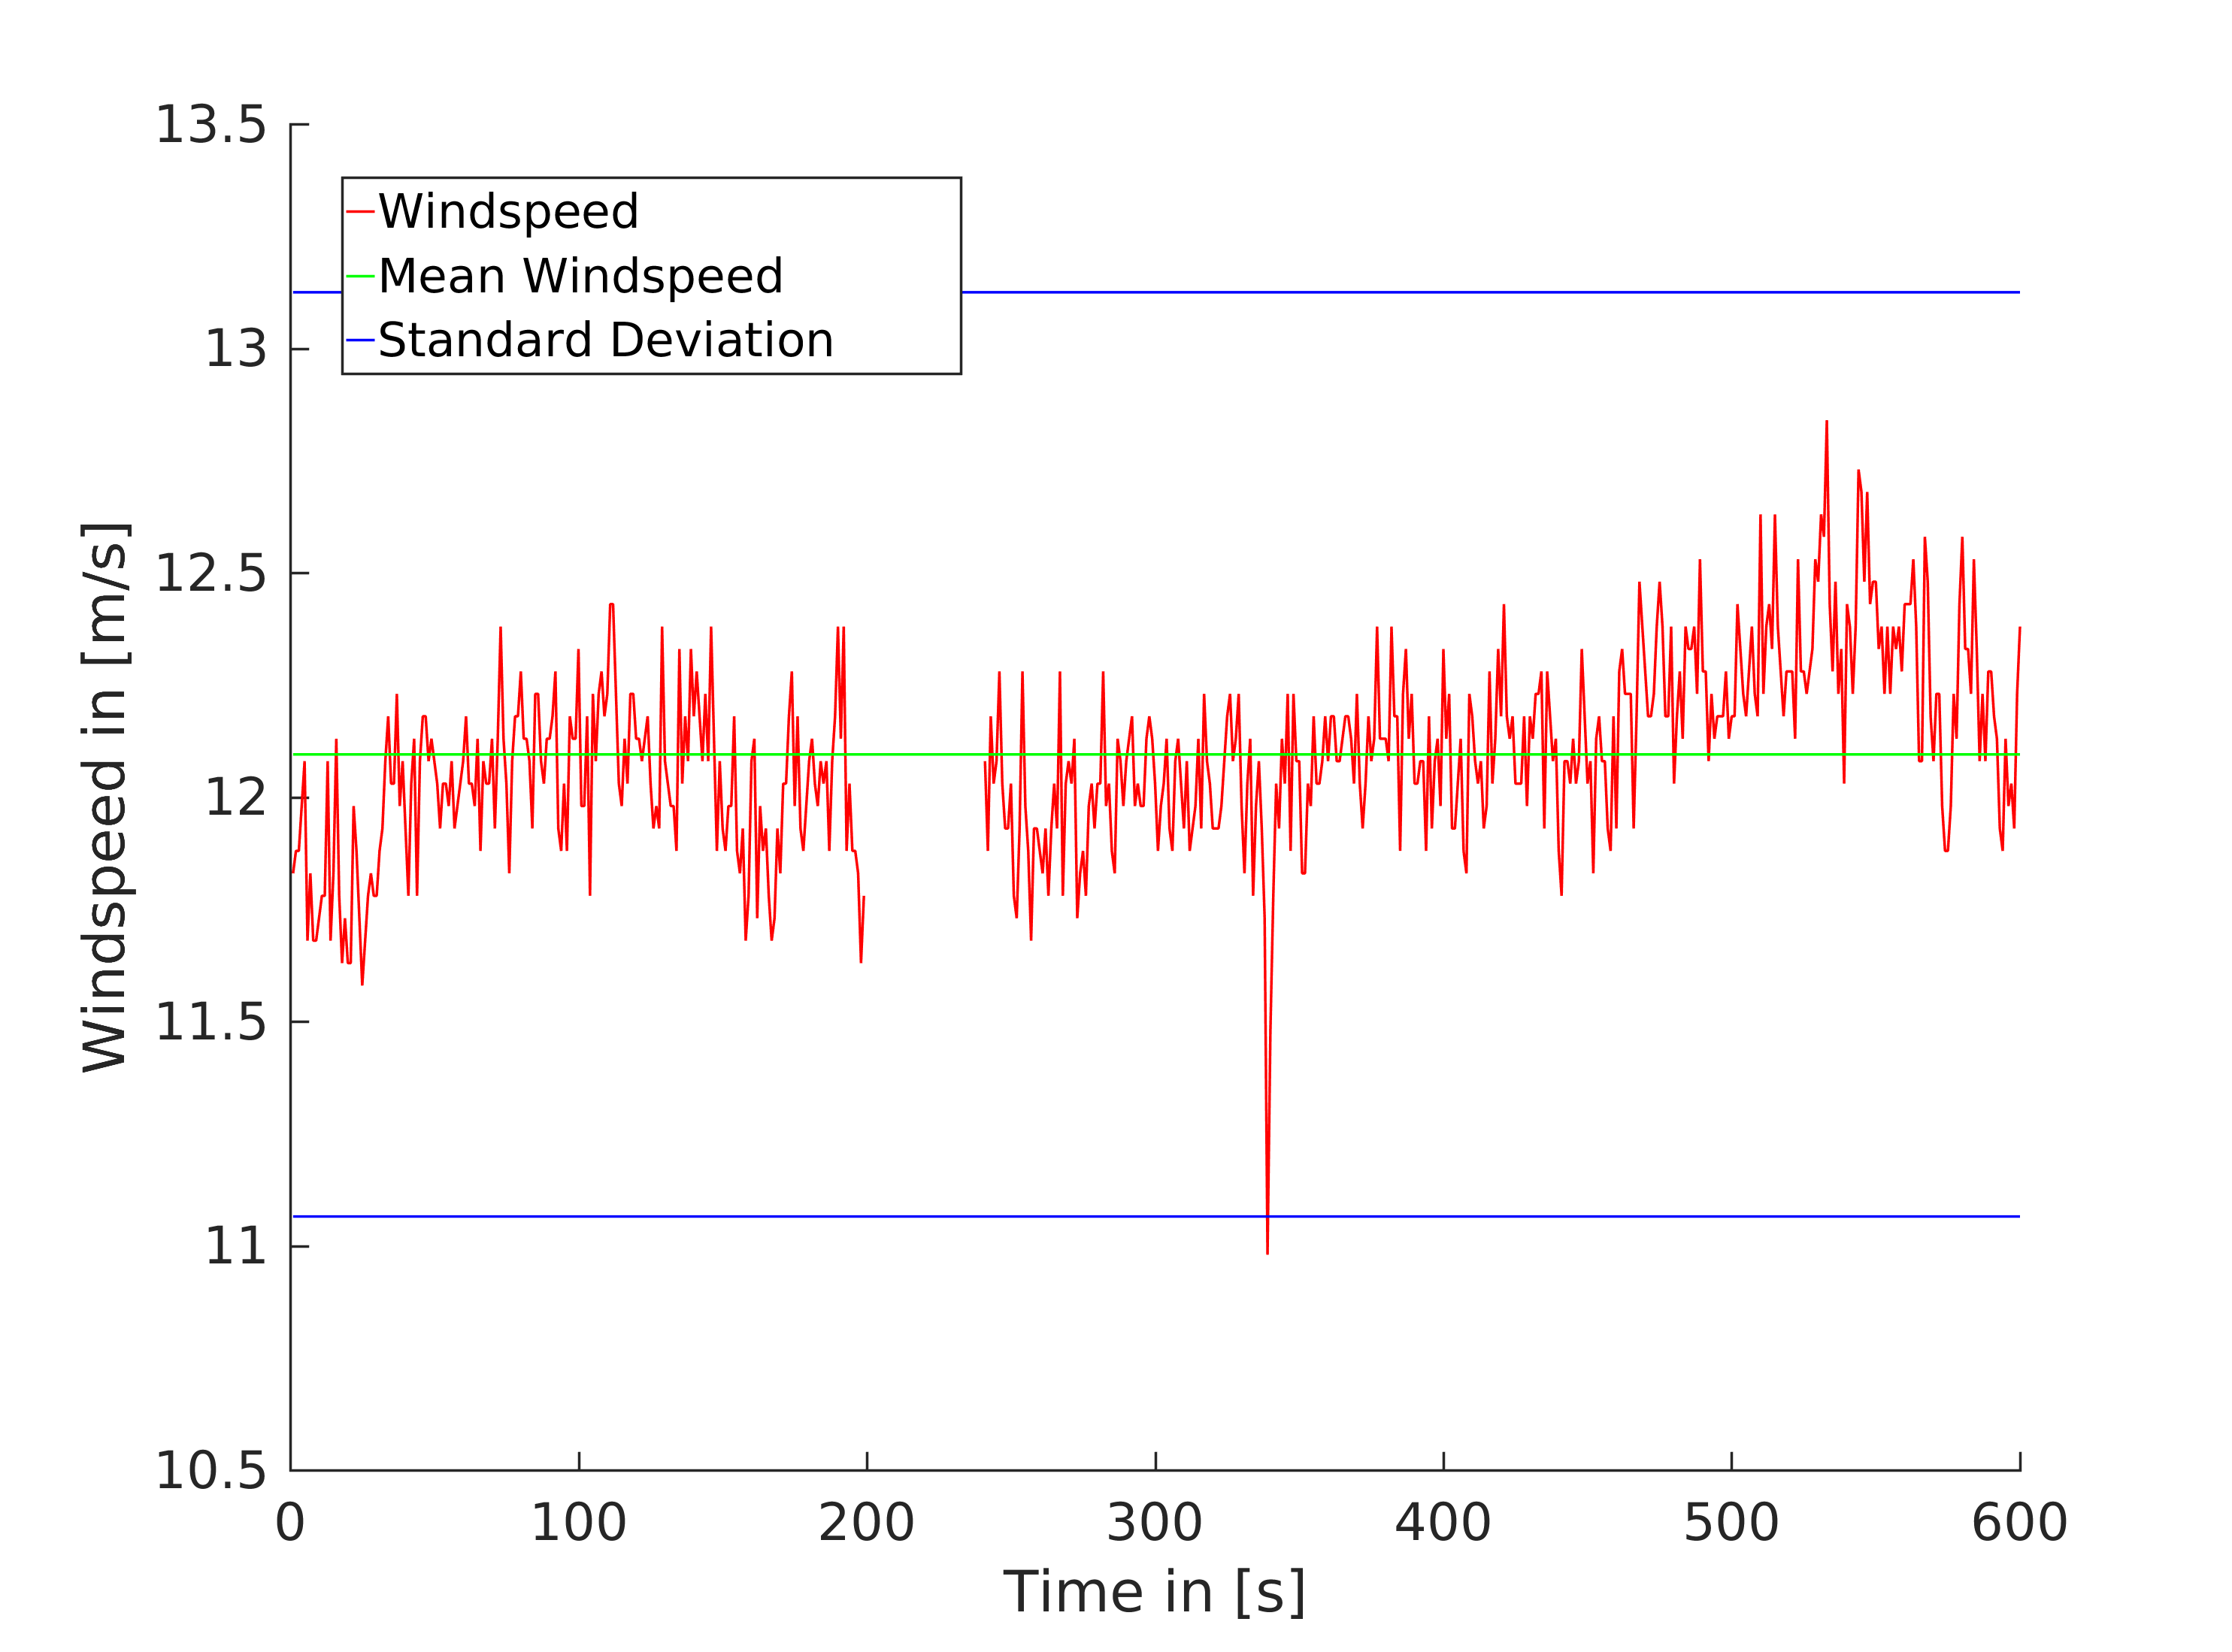
\includegraphics[width=1\linewidth]{../Plots/spikesintervall440.png}
  \caption{Unphysical cause}
  \label{fig:spikeUnphys}
\end{figure}

All in all we can say that the $5\sigma$ criterion is only an estimation of unusable values and relies on experience. By fixing the threshold to $5\sigma$ one states that all fluctuation within this interval are statistically significant. It implies reliability of the measurement system and is vulnerable enviromental influences, e.g. weather conditions.

\section{Increment PDF}
In this last task the increment PDF was to be computed. This probability density defines the distribution of short term changes on the time axis in the data. The formalism is $\delta u_{\tau} = u(t+\tau)-u(t)$ for a time lag of $\tau=1s$. We collected the data in a histogram with $100$ bins and normalized the values to unit standard deviation.
\begin{figure}[htb!]
  \centering
  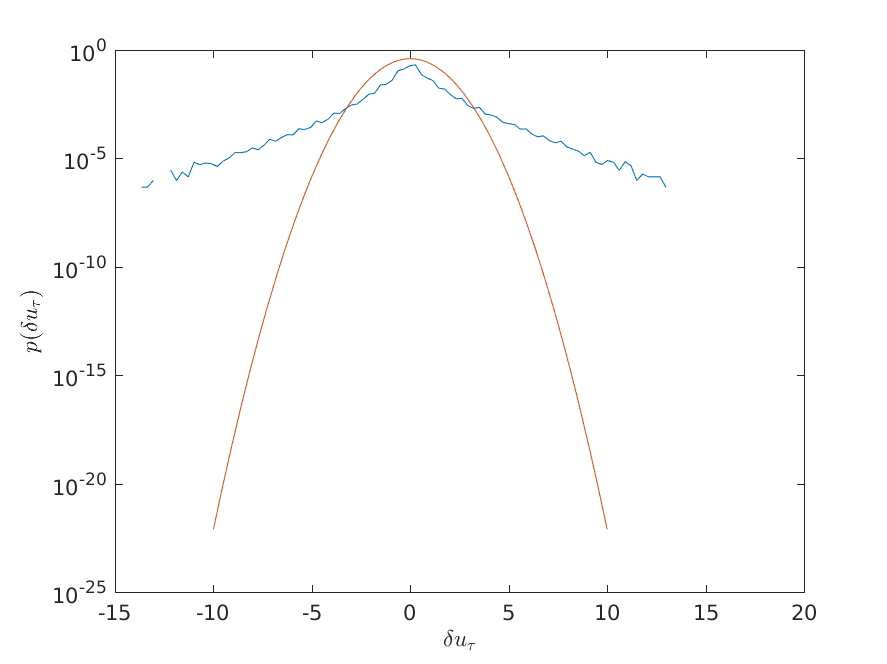
\includegraphics[width=1\linewidth]{../Plots/tau_pdf_gauss10.png}
  \caption{Unphysical cause}
  \label{fig:incrementPdf}
\end{figure}

\end{document}